\subsection{Temporal Modeling}
\label{sec:temporal}
Temporal consistency is not the requirement that adjacent frames look alike. It requires that changes agree with motion, occlusion, illumination, and scene structure. A static-background assumption can be useful in one region and wrong in another. A model must preserve actual motion while suppressing unexplained appearance changes. Figure~\ref{fig:temporal} shows how two representative systems implement this requirement. StableVSR obtains texture guidance from a motion-compensated neighboring reconstruction, whereas Upscale-A-Video combines local temporal modules, recurrent propagation across segments, and temporal decoding. The location and reach of information exchange determine which temporal errors each design can address.

\begin{figure*}[t]
\centering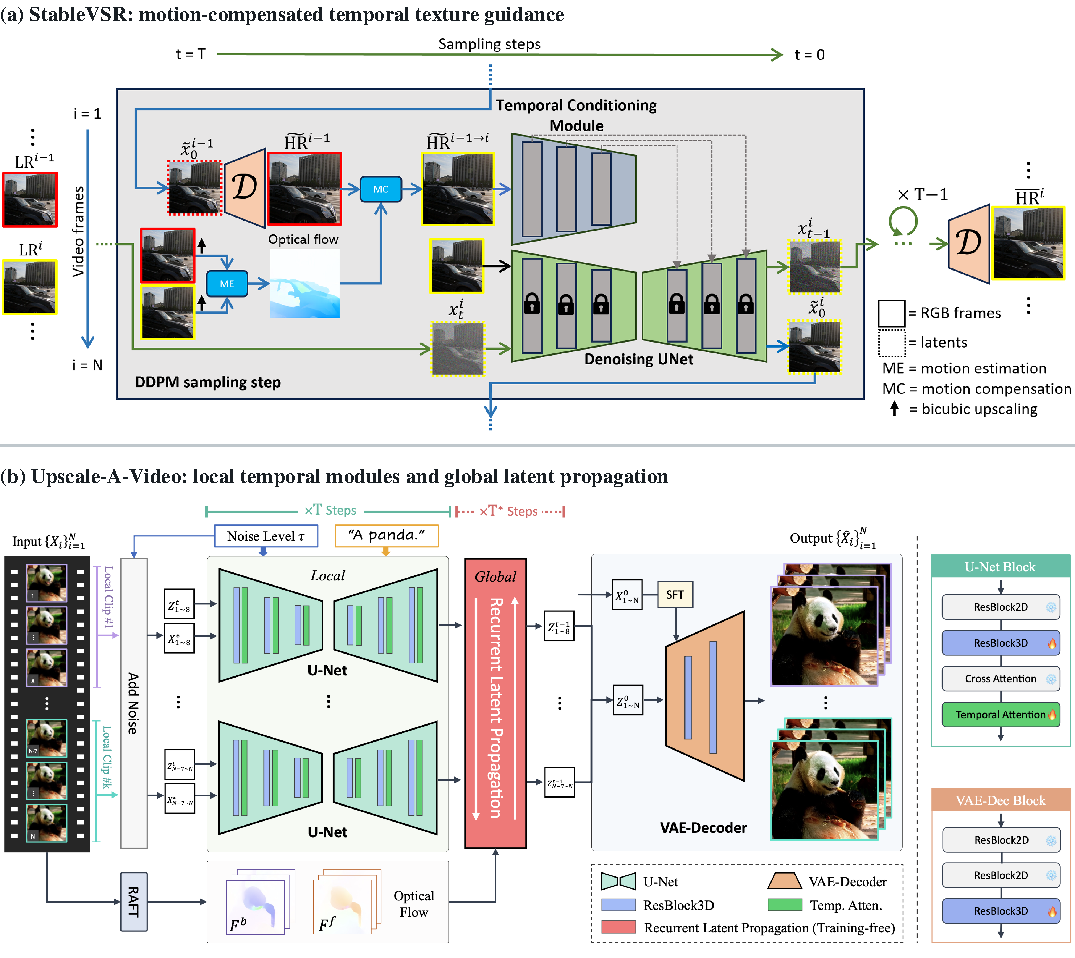
\includegraphics[width=\textwidth]{figures/temporal_mechanisms.pdf}
\caption{Concrete architectures for temporal modeling, reproduced from the original papers under \href{https://creativecommons.org/licenses/by/4.0/}{CC BY 4.0}. (a) StableVSR~\cite{stablevsr}, Fig.~2: optical flow warps reconstructed texture from a neighboring frame, and a temporal conditioning module guides the frozen denoising U-Net. (b) Upscale-A-Video~\cite{upscale}, Fig.~2: temporal layers model local clips, bidirectional recurrent latent propagation exchanges information across clips at selected diffusion steps, and a finetuned VAE decoder improves RGB consistency. Original module names and frozen/trainable annotations are retained.}
\label{fig:temporal}
\end{figure*}

\subsubsection{Noise Coupling and Initialization}
Independent framewise sampling allows each frame to choose a different plausible explanation of missing texture. Sharing, correlating, or propagating initial noise reduces this source of variation~\cite{zvrd}. However, identical image-coordinate noise is not identical object-coordinate noise when the camera or object moves. A texture can remain fixed to the screen rather than to a surface. Motion-aware noise propagation is a more appropriate conceptual target, but resampling changes noise statistics and requires a policy for disoccluded regions.

Initialization also controls how much a video changes. Noise Calibration constrains the starting noise of a pretrained video diffusion model to preserve source content~\cite{ncsdedit}. Inpainting methods can initialize from a coarse, temporally coherent completion rather than pure noise~\cite{diffueraser}. These choices restrict the space explored by the generator, but they can also preserve errors in the initialization. The relevant question is not merely whether frames become more similar; it is whether the initialization supports correct detail and motion after refinement.

Warped Diffusion~\cite{warped} first adapts SDXL to conditional image restoration, including training with correlated Gaussian-process noise. It then warps a continuous noise field according to motion and uses inference-time equivariance self-guidance to align denoiser predictions across frames. Its central insight is that correlated inputs alone do not guarantee correlated outputs: the denoiser must also behave consistently under the corresponding transformation. The resulting model transfers image restoration knowledge to video without learning from video training pairs.

\subsubsection{Correspondence and Motion-Guided Propagation}
Given estimated correspondence $u_{t-1\rightarrow t}$ and an occlusion-validity mask $M_t$, a typical temporal penalty is
\begin{equation}
\mathcal L_{\mathrm{warp}}=
\frac{\sum_t\|M_t\odot[\widehat x_t-\mathcal W(\widehat x_{t-1},u_{t-1\rightarrow t})]\|_1}
{\sum_t\|M_t\|_1+\varepsilon},
\label{eq:warp}
\end{equation}
where $\mathcal W$ warps a preceding frame into the current coordinates. Related constraints can act on features or latents rather than RGB output. Upscale-A-Video combines temporal modules with flow-guided latent propagation; StableVSR uses temporal conditioning and texture guidance; MGLD-VSR introduces motion guidance into the diffusion trajectory~\cite{upscale,stablevsr,mgld}. DiffIR2VR-Zero transfers information with hierarchical latent warping and token merging~\cite{diffir2vr}.

These approaches use observed redundancy to constrain ambiguity, but correspondence is least reliable precisely where restoration is hardest: heavy blur, low light, rain, repetitive texture, large motion, and occlusion. Warping a wrong texture consistently can improve a temporal score while reducing fidelity. Confidence weighting and disocclusion handling are therefore central, not minor implementation details. At motion boundaries, the flow estimator and restoration model interact: improving propagation requires both accurate correspondence and protection against invalid matches.

Long-range propagation adds a second failure mode. Information reused across many frames can preserve identity through temporary occlusion, but an early hallucination can also become persistent state. Local coherence is not evidence of globally correct reconstruction. Scene-cut resets, confidence-weighted updates, and re-anchoring to current observations can limit error accumulation over long clips.

Temporal consistency depends on which information is propagated and where it enters the restoration process. Dense motion alignment, instance-level semantics, and learned video dynamics provide different forms of temporal support. DGAF-VSR revisits feature compensation inside a diffusion pipeline: its Optical Guided Warping Module aligns features through an upscale--warp--downscale operation, while its Feature-wise Temporal Condition Module supplies dense guidance from neighboring frames~\cite{dgaf}. This design seeks to preserve useful high-frequency evidence before the generative model supplies missing detail; the reported benefit of increasing the warping resolution is not monotonic. Semantic correspondence offers another route when local appearance is unreliable. SeeClear couples instance-centric clip alignment and a channel-wise texture memory with a frozen OpenSeeD semantic distiller~\cite{seeclear}. Its blurring ResShift process operates on discrete-wavelet subbands, avoiding a learned autoencoder; the DCT-based blur construction and DWT-based representation serve distinct purposes. SeTe-VSR instead injects SAM2 semantic embeddings and temporal-spatial awareness into an SD2.1-based latent denoiser and augments the VAE decoder with temporal layers~\cite{setevsr}. These approaches illustrate that temporal support can reside in aligned observations, object-level representations, or the reconstruction decoder. The resulting mechanisms address different failure modes: flow alignment depends on correspondence accuracy, semantic alignment depends on object representations, and decoder adaptation targets the conversion of coherent features into stable pixels.

\subsubsection{Temporal Layers, Attention, and Memory}
Learned temporal convolution, recurrent modules, state-space components, and temporal attention allow features from multiple frames to influence denoising. These mechanisms can be trained as additions to an image prior or inherited from a video prior~\cite{upscale,scst,star}. The distinction affects both data requirements and the source of improvement. An added temporal block learns motion from restoration data, whereas a video foundation model has already absorbed a motion distribution during pretraining.

Attention supports interaction beyond explicit flow, but it does not guarantee correct correspondence. Similar-looking regions may exchange incompatible details, and global attention can become expensive at high spatial and temporal resolution. Windowed attention limits cost but introduces a new requirement: information must cross window boundaries in a controlled way. SeedVR's shifted variable-size windows and DC-VSR's spatial and temporal attention propagation exemplify mechanisms for extending processing beyond the native support of a backbone~\cite{seedvr,dcvsr}.

Memory and cached keys/values can preserve context while reducing repeated computation. Their correctness depends on how cached features align with the current denoising state and frame positions. A cache designed for autoregressive synthesis cannot be assumed to preserve restoration fidelity under arbitrary input changes. Streaming VSR methods consequently combine cache or propagation strategies with observation-conditioned restoration~\cite{stream,infvsr,flash}. Their central difficulty is keeping cached context useful under accumulated drift, abrupt motion, and scene transitions.

\subsubsection{Losses and the Decoder}
Temporal losses may act on warped RGB frames, deep features, motion-compensated residuals, or discriminator features. They encourage different invariances. A pixel penalty strongly preserves aligned intensities but may penalize true lighting change; a feature penalty can tolerate some appearance variation but miss fine flicker. An adversarial temporal loss can promote plausible dynamics without ensuring that those dynamics match the observed scene. No single loss should be equated with complete temporal correctness.

The decoder is a separate source of temporal error. Consistent latents can produce unstable high-frequency RGB detail if decoded independently. Temporal-aware decoding in MGLD-VSR and conditional or lightweight decoding in efficient methods make this issue explicit~\cite{mgld,flash}. This creates a second temporal modeling stage after denoising. Its interaction with spatial tiling and temporal chunking becomes particularly important when high-resolution videos exceed the decoder's native processing window.

\subsubsection{Comparison of Temporal Mechanisms}
\begin{table*}[t]
\caption{Comparison of temporal mechanisms, the information they constrain, and their characteristic challenges.}
\label{tab:temporal}\centering\footnotesize
\begin{tabularx}{\textwidth}{@{}p{0.18\textwidth}YYY@{}}\toprule
Mechanism & Representative use & What it constrains & Main challenge \\\midrule
Shared or calibrated noise & ZVRD; Noise Calibration~\cite{zvrd,ncsdedit} & Random variation or initial deviation from the source & Moving textures; scene cuts; several random seeds \\
Flow/latent propagation & Upscale-A-Video; MGLD-VSR; DiffIR2VR-Zero~\cite{upscale,mgld,diffir2vr} & Appearance along estimated correspondences & Disocclusion; incorrect flow; large motion; repetitive patterns \\
Temporal conditioning & StableVSR; FLAIR~\cite{stablevsr,flair} & Cross-frame feature and texture relationships & Long occlusion; identity changes; frame-rate shifts \\
Joint/windowed attention & STAR; SeedVR; DC-VSR~\cite{star,seedvr,dcvsr} & Contextual dependencies across frames or partitions & Window boundaries; native-context overflow; persistent objects \\
State/cache reuse & Stream-DiffVSR; InfVSR~\cite{stream,infvsr} & Recurrent context under bounded computation & Long-horizon drift; stale state; abrupt content change \\
Temporal decoding & MGLD-VSR; FlashVSR~\cite{mgld,flash} & Mapping from latent consistency to RGB consistency & Fine textures; tiled decoding; chunk boundaries \\\bottomrule
\end{tabularx}
\end{table*}

Table~\ref{tab:temporal} reveals complementary roles for these mechanisms. Noise coupling limits stochastic variation before reconstruction, while correspondence constrains geometric consistency along visible trajectories. Attention aggregates evidence beyond explicit pairwise warps, and memory extends that evidence over longer intervals. Temporal decoding then preserves the resulting latent consistency in pixel space. Combining these mechanisms can address different sources of flicker, but their errors can also interact: unreliable flow can contaminate memory, and an incoherent decoder can erase gains made by the denoiser.
